\documentclass[11pt]{article}

% ---------------- Packages ----------------
\usepackage[margin=1in]{geometry}
\usepackage{amsmath,amssymb,amsthm}
\usepackage{graphicx}
\usepackage{hyperref}
\usepackage{fancyhdr}
\usepackage{enumitem}
\usepackage[UTF8]{ctex}
\usepackage{algorithm}
\usepackage{algpseudocode}
% ---------------- Header ----------------
\pagestyle{fancy}
\fancyhf{}
\lhead{Course Name}
\rhead{Homework \#1}
\cfoot{\thepage}

% ---------------- Title ----------------
\title{Homework 1}
\author{羊瑞 \\ 2300013091}
\date{\today}

% ---------------- Custom commands ----------------
\newcommand{\R}{\mathbb{R}}
\newcommand{\E}{\mathbb{E}}

% ---------------- Problem Environment ----------------
\newcounter{problem}

\newenvironment{problem}[1][]{
\stepcounter{problem}
\section*{Problem \theproblem\; #1}
}{}

\newenvironment{solution}{
\par\noindent\textbf{Solution.}\par\noindent
}{\qed}

\setlength{\parindent}{0pt}
% ---------------- Document ----------------
\begin{document}

\maketitle

\begin{problem} 
\begin{center}
    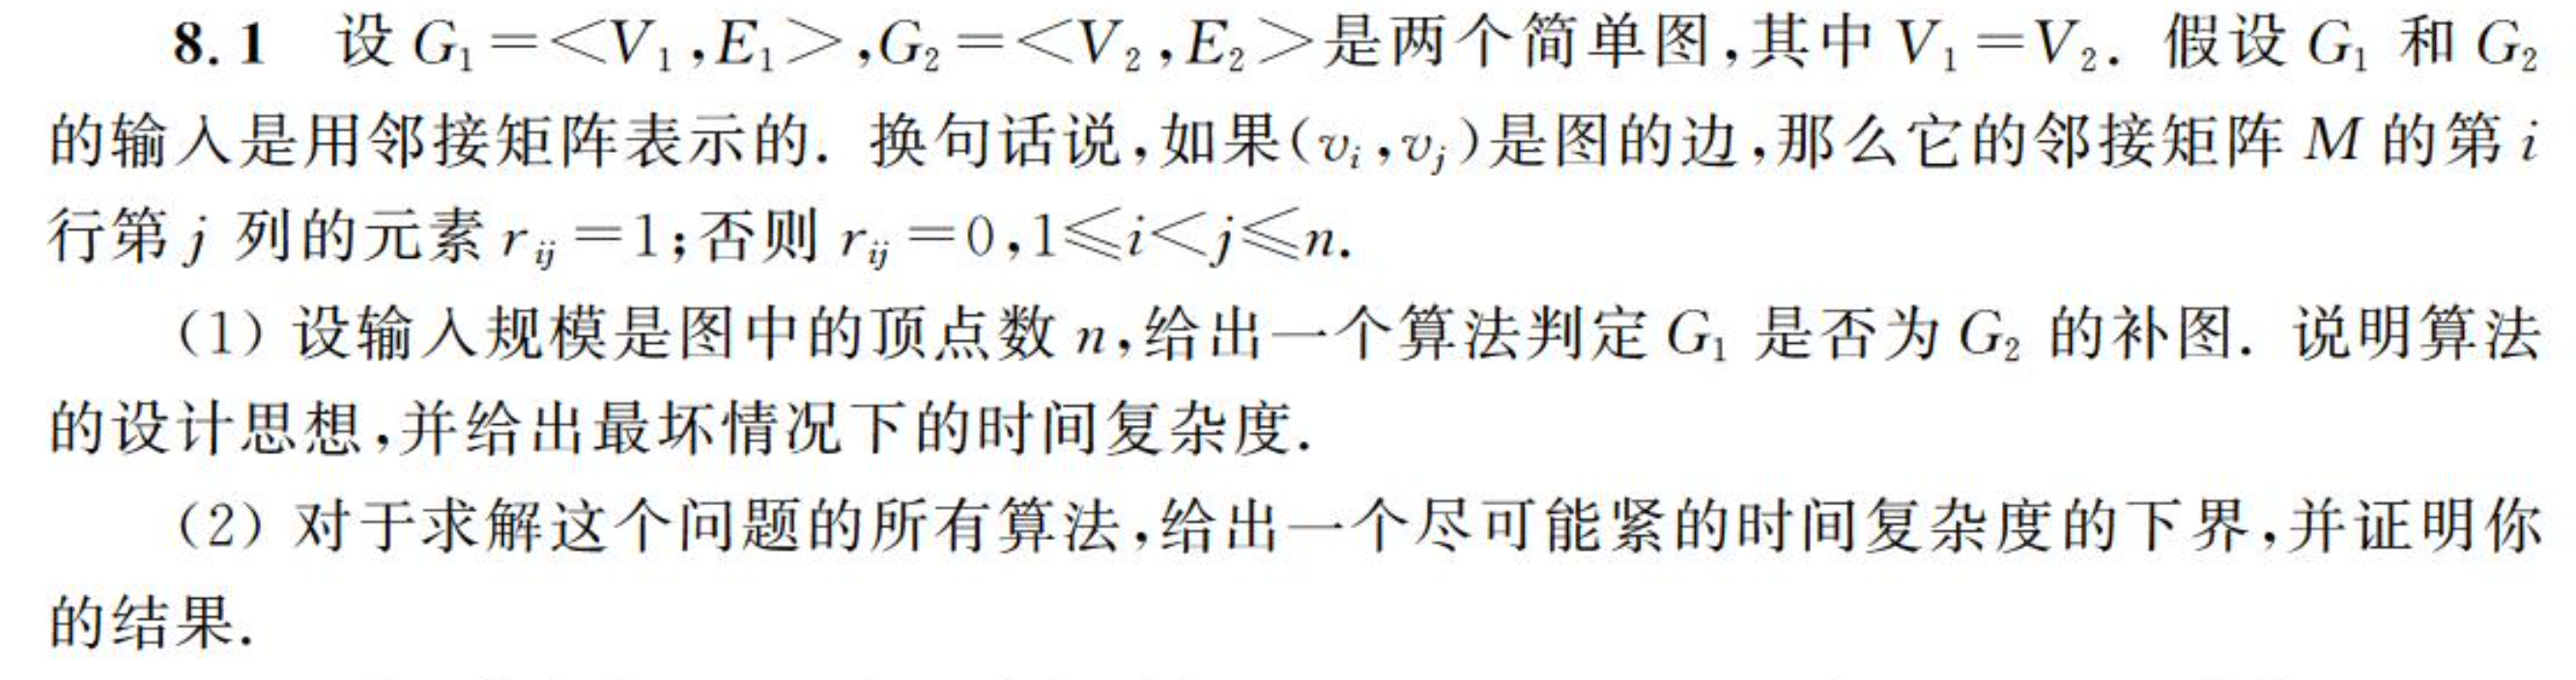
\includegraphics[width=0.6\textwidth]{problems/8.1.png}
\end{center}
\end{problem}

\begin{solution}
(1) 算法设计

设 $M_1$ 和 $M_2$ 分别是 $G_1$ 和 $G_2$ 的邻接矩阵。若 $G_1$ 是 $G_2$ 的补图，则对于任意不同顶点 $v_i,v_j$，边 $(v_i,v_j)$ 在 $G_1$ 中存在当且仅当它不在 $G_2$ 中存在。

也就是说，对任意
\[
1\leq i<j\leq n,
\]
都应该有
\[
M_1[i][j]+M_2[i][j]=1.
\]

因此可以直接检查两个邻接矩阵中每一对对应元素是否互补。

算法如下：

\[
\begin{array}{l}
\textbf{Complement-Check}(M_1,M_2,n):\\
\quad \textbf{for } i=1 \textbf{ to } n-1 \textbf{ do}\\
\quad\quad \textbf{for } j=i+1 \textbf{ to } n \textbf{ do}\\
\quad\quad\quad \textbf{if } M_1[i][j]+M_2[i][j]\neq 1 \textbf{ then}\\
\quad\quad\quad\quad \textbf{return false}\\
\quad \textbf{return true}
\end{array}
\]

算法思想是：逐一检查每一对不同顶点之间的边是否在两个图中恰好出现一次。如果某一条边在两个图中都出现，或者都不出现，则 $G_1$ 不是 $G_2$ 的补图。

需要检查的顶点对数量为

\[
\binom{n}{2}=\frac{n(n-1)}{2}.
\]

每次检查只需要常数时间，因此最坏情况下时间复杂度为

\[
T(n)=\Theta\left(\binom{n}{2}\right)=\Theta(n^2).
\]

(2) 时间复杂度下界证明

下面证明任何求解该问题的算法在最坏情况下都需要

\[
\Omega(n^2)
\]

时间。

对于 $n$ 个顶点的简单图，需要考虑的无序顶点对数量为

\[
\binom{n}{2}.
\]

对每一对顶点 $(v_i,v_j)$，其中 $i<j$，算法必须判断

\[
M_1[i][j]+M_2[i][j]=1
\]

是否成立。

假设存在一个正确算法，在某一次运行中没有检查某一对顶点 $(v_p,v_q)$ 对应的元素。也就是说，它没有获得关于

\[
M_1[p][q]
\quad \text{和} \quad
M_2[p][q]
\]

是否互补的充分信息。

考虑一个输入实例，其中 $G_1$ 是 $G_2$ 的补图。此时对所有 $i<j$ 都有

\[
M_1[i][j]+M_2[i][j]=1.
\]

现在只改变未被检查的这一对顶点对应的某个矩阵元素。例如保持其他所有元素不变，只把

\[
M_1[p][q]
\]

从 $0$ 改成 $1$，或者从 $1$ 改成 $0$。由于 $x$ 未被算法检查，算法在两个输入上的执行过程完全相同，因此会给出相同的输出。

但是修改之后，在顶点对 $(v_p,v_q)$ 上有

\[
M_1[p][q]+M_2[p][q]\neq 1,
\]

所以修改后的两个图不再互为补图。

这就得到两个输入：
一个是互补图实例，另一个不是互补图实例，

但算法无法区分它们，矛盾。

因此，任何正确算法在最坏情况下都必须检查所有顶点对，至少需要

\[
\binom{n}{2}=\frac{n(n-1)}{2}
\]

次基本检查。

所以任意算法的最坏时间复杂度都有下界

\[
T(n)=\Omega(n^2).
\]

结合第 $(1)$ 问中的算法可知，该问题的最优最坏时间复杂度为

\[
\Theta(n^2).
\]
\end{solution}

\begin{problem}
\begin{center}
    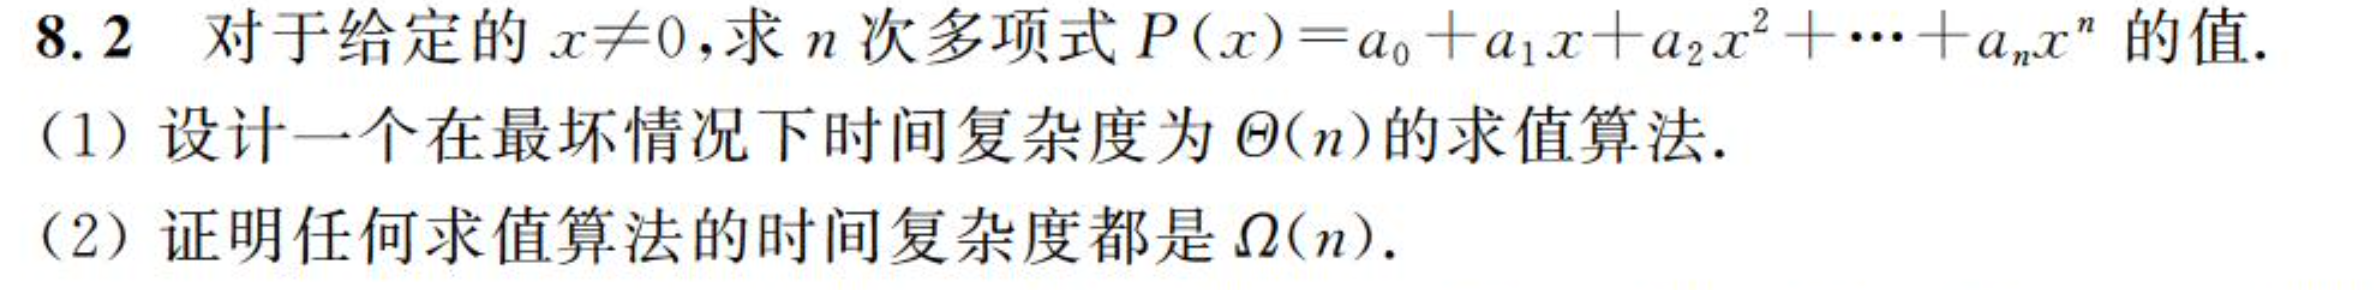
\includegraphics[width=0.6\textwidth]{problems/8.2.png}
\end{center}
\end{problem}

\begin{solution}

(1) 算法设计
\[
P(x)=a_0+x\bigl(a_1+x(a_2+\cdots+x(a_{n-1}+xa_n)\cdots)\bigr).
\]

令

\[
b\leftarrow a_n.
\]

然后依次计算

\[
b\leftarrow a_k+xb,\qquad k=n-1,n-2,\ldots,0.
\]

最后输出

\[
b=P(x).
\]

伪代码为：

\[
\begin{array}{l}
b\leftarrow a_n,\\
\text{for } k=n-1 \text{ downto } 0 \text{ do}\\
\qquad b\leftarrow a_k+xb,\\
\text{return } b.
\end{array}
\]

该算法循环执行 $n$ 次，每次只进行一次乘法和一次加法，因此最坏情况下时间复杂度为

\[
T(n)=\Theta(n).
\]

(2) 下界证明

因为多项式共有

\[
a_0,a_1,\ldots,a_n
\]

这 $n+1$ 个系数。任意正确算法必须至少读取所有系数。

否则，假设某个系数 $a_i$ 没有被读取。则可以构造两个多项式

\[
P_1(x)=a_0+\cdots+a_ix^i+\cdots+a_nx^n,
\]

\[
P_2(x)=a_0+\cdots+a_i'x^i+\cdots+a_nx^n,
\qquad a_i'\neq a_i.
\]

这两个多项式除第 $i$ 个系数外完全相同。由于算法没有读取 $a_i$，所以算法无法区分 $P_1$ 和 $P_2$，会给出相同输出。

但是由于 $x\neq 0$，有

\[
P_1(x)-P_2(x)=(a_i-a_i')x^i\neq 0.
\]

因此

\[
P_1(x)\neq P_2(x),
\]

这与算法正确性矛盾。

所以任何正确算法都必须至少读取 $n+1$ 个系数，因而时间复杂度至少为

\[
\Omega(n).
\]

结合第 $(1)$ 问中的算法可知，多项式求值问题的最优时间复杂度为

\[
\Theta(n).
\]
\end{solution}

\begin{problem}
\begin{center}
    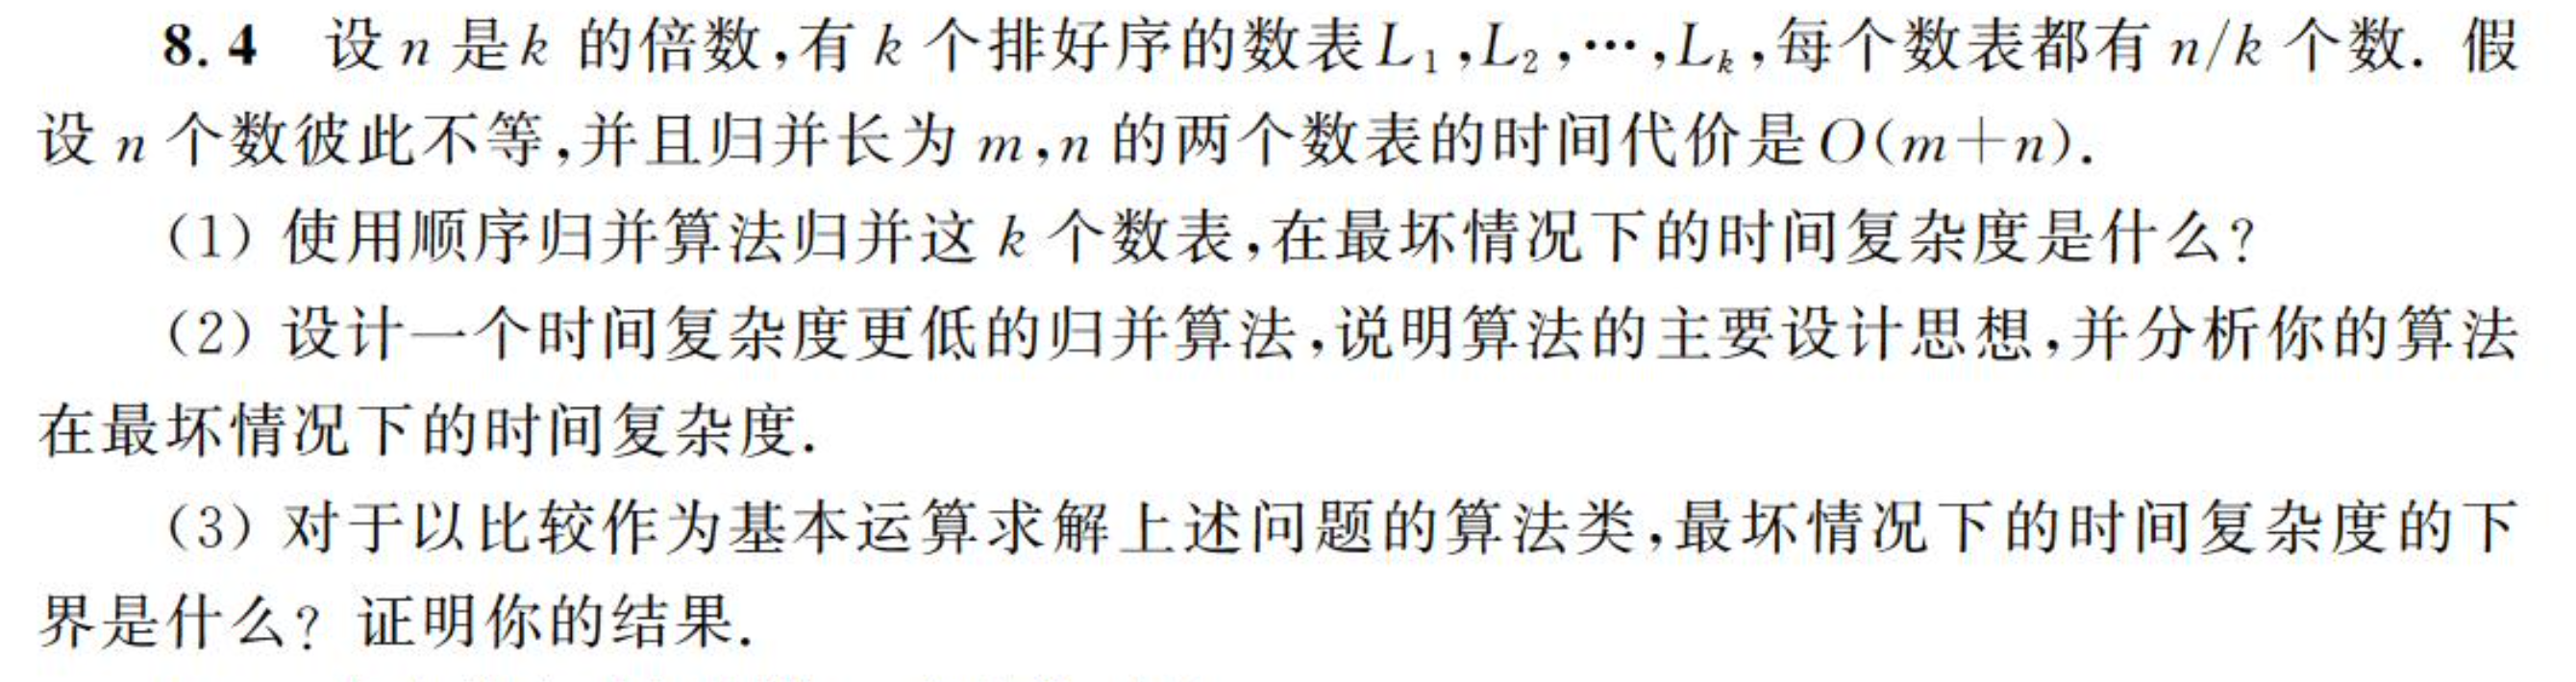
\includegraphics[width=0.6\textwidth]{problems/8.4.png}
\end{center}
\end{problem}

\begin{solution}
(1)
顺序归并的做法是：

\[
(((L_1\cup L_2)\cup L_3)\cup \cdots \cup L_k).
\]
第 $i$ 次归并的总长度为

\[
\frac{(i+1)n}{k}.
\]

因此总时间为

\[
T(n,k)
=
O\left(
\frac{2n}{k}
+\frac{3n}{k}
+\cdots
+\frac{kn}{k}
\right).
\]

于是

\[
T(n,k)
=
O\left(
\frac{n}{k}\sum_{i=2}^{k} i
\right).
\]

所以

\[
T(n,k)
=
O\left(
\frac{n}{k}\cdot k^2
\right)
=
O(nk).
\]

因此，顺序归并算法在最坏情况下的时间复杂度为

\[
O(nk).
\]

更准确地说，其时间复杂度为

\[
\Theta(nk).
\]
(2)

采用分治归并算法。
每次把当前所有有序表两两归并，形成更长的有序表。重复这一过程，直到只剩下一个有序表。

第一轮：

\[
L_1 \text{ 与 } L_2 \text{ 归并},\quad
L_3 \text{ 与 } L_4 \text{ 归并},\quad \ldots
\]

第二轮：把第一轮得到的有序表继续两两归并。

如此反复。

伪代码如下：

\[
\begin{array}{l}
\textbf{Merge-K-Lists}(L_1,L_2,\ldots,L_k):\\
\quad \textbf{while } k>1 \textbf{ do}\\
\quad\quad \text{将当前所有有序表两两归并}\\
\quad\quad \text{若有一个表落单，则直接进入下一轮}\\
\quad \textbf{return } \text{最后剩下的有序表}
\end{array}
\]

每一轮中，每个元素最多参与一次归并。因此，每一轮的总代价为

\[
O(n).
\]

每经过一轮，表的个数大约减半，所以总共需要

\[
\lceil \log_2 k\rceil
\]

轮。

因此总时间复杂度为

\[
T(n,k)=O(n\log k).
\]

所以该算法在最坏情况下的时间复杂度为

\[
O(n\log k).
\]

这比顺序归并的

\[
O(nk)
\]

更低。

(3)

下面证明：对于以比较作为基本运算的算法类，最坏情况下时间复杂度下界为

\[
\Omega(n\log k).
\]

因为每个有序表内部的相对顺序已经确定，所以算法真正需要确定的是：这 $k$ 个有序表中的元素在最终有序序列中的交错方式。

每个表有

\[
\frac{n}{k}
\]

个元素，因此不同的合法交错方式数量为多项式系数

\[
N
=
\binom{n}{\frac{n}{k},\frac{n}{k},\ldots,\frac{n}{k}}
=
\frac{n!}{\left(\left(\frac{n}{k}\right)!\right)^k}.
\]

任何基于比较的算法都可以看成一棵决策树。若算法能够正确区分所有可能的输入情况，则这棵决策树至少要有

\[
N
\]

个叶子结点。

若最坏情况下需要比较 $h$ 次，则决策树高度为 $h$，叶子数最多为

\[
2^h.
\]

因此必须有

\[
2^h \geq N.
\]

于是

\[
h\geq \log_2 N.
\]

下面估计 $\log_2 N$：

\[
\log_2 N
=
\log_2 n!
-
k\log_2\left(\frac{n}{k}!\right).
\]

由 Stirling 公式，

\[
\log_2 n! = \Theta(n\log n),
\]

并且

\[
\log_2\left(\frac{n}{k}!\right)
=
\Theta\left(\frac{n}{k}\log\frac{n}{k}\right).
\]

所以

\[
\begin{aligned}
\log_2 N
&=
\Theta(n\log n)
-
k\cdot
\Theta\left(\frac{n}{k}\log\frac{n}{k}\right)\\
&=
\Theta(n\log n)
-
\Theta\left(n\log\frac{n}{k}\right)\\
&=
\Theta\left(n\log n-n\log\frac{n}{k}\right)\\
&=
\Theta(n\log k).
\end{aligned}
\]

因此，任何基于比较的归并算法在最坏情况下至少需要

\[
\Omega(n\log k)
\]

次比较。

即

\[
T(n,k)=\Omega(n\log k).
\]

结合第 $(2)$ 问中的分治归并算法，其最坏情况下时间复杂度为

\[
O(n\log k),
\]

因此该问题在比较模型下的最优最坏时间复杂度为

\[
\Theta(n\log k).
\]
\end{solution}

\begin{problem}
\begin{center}
    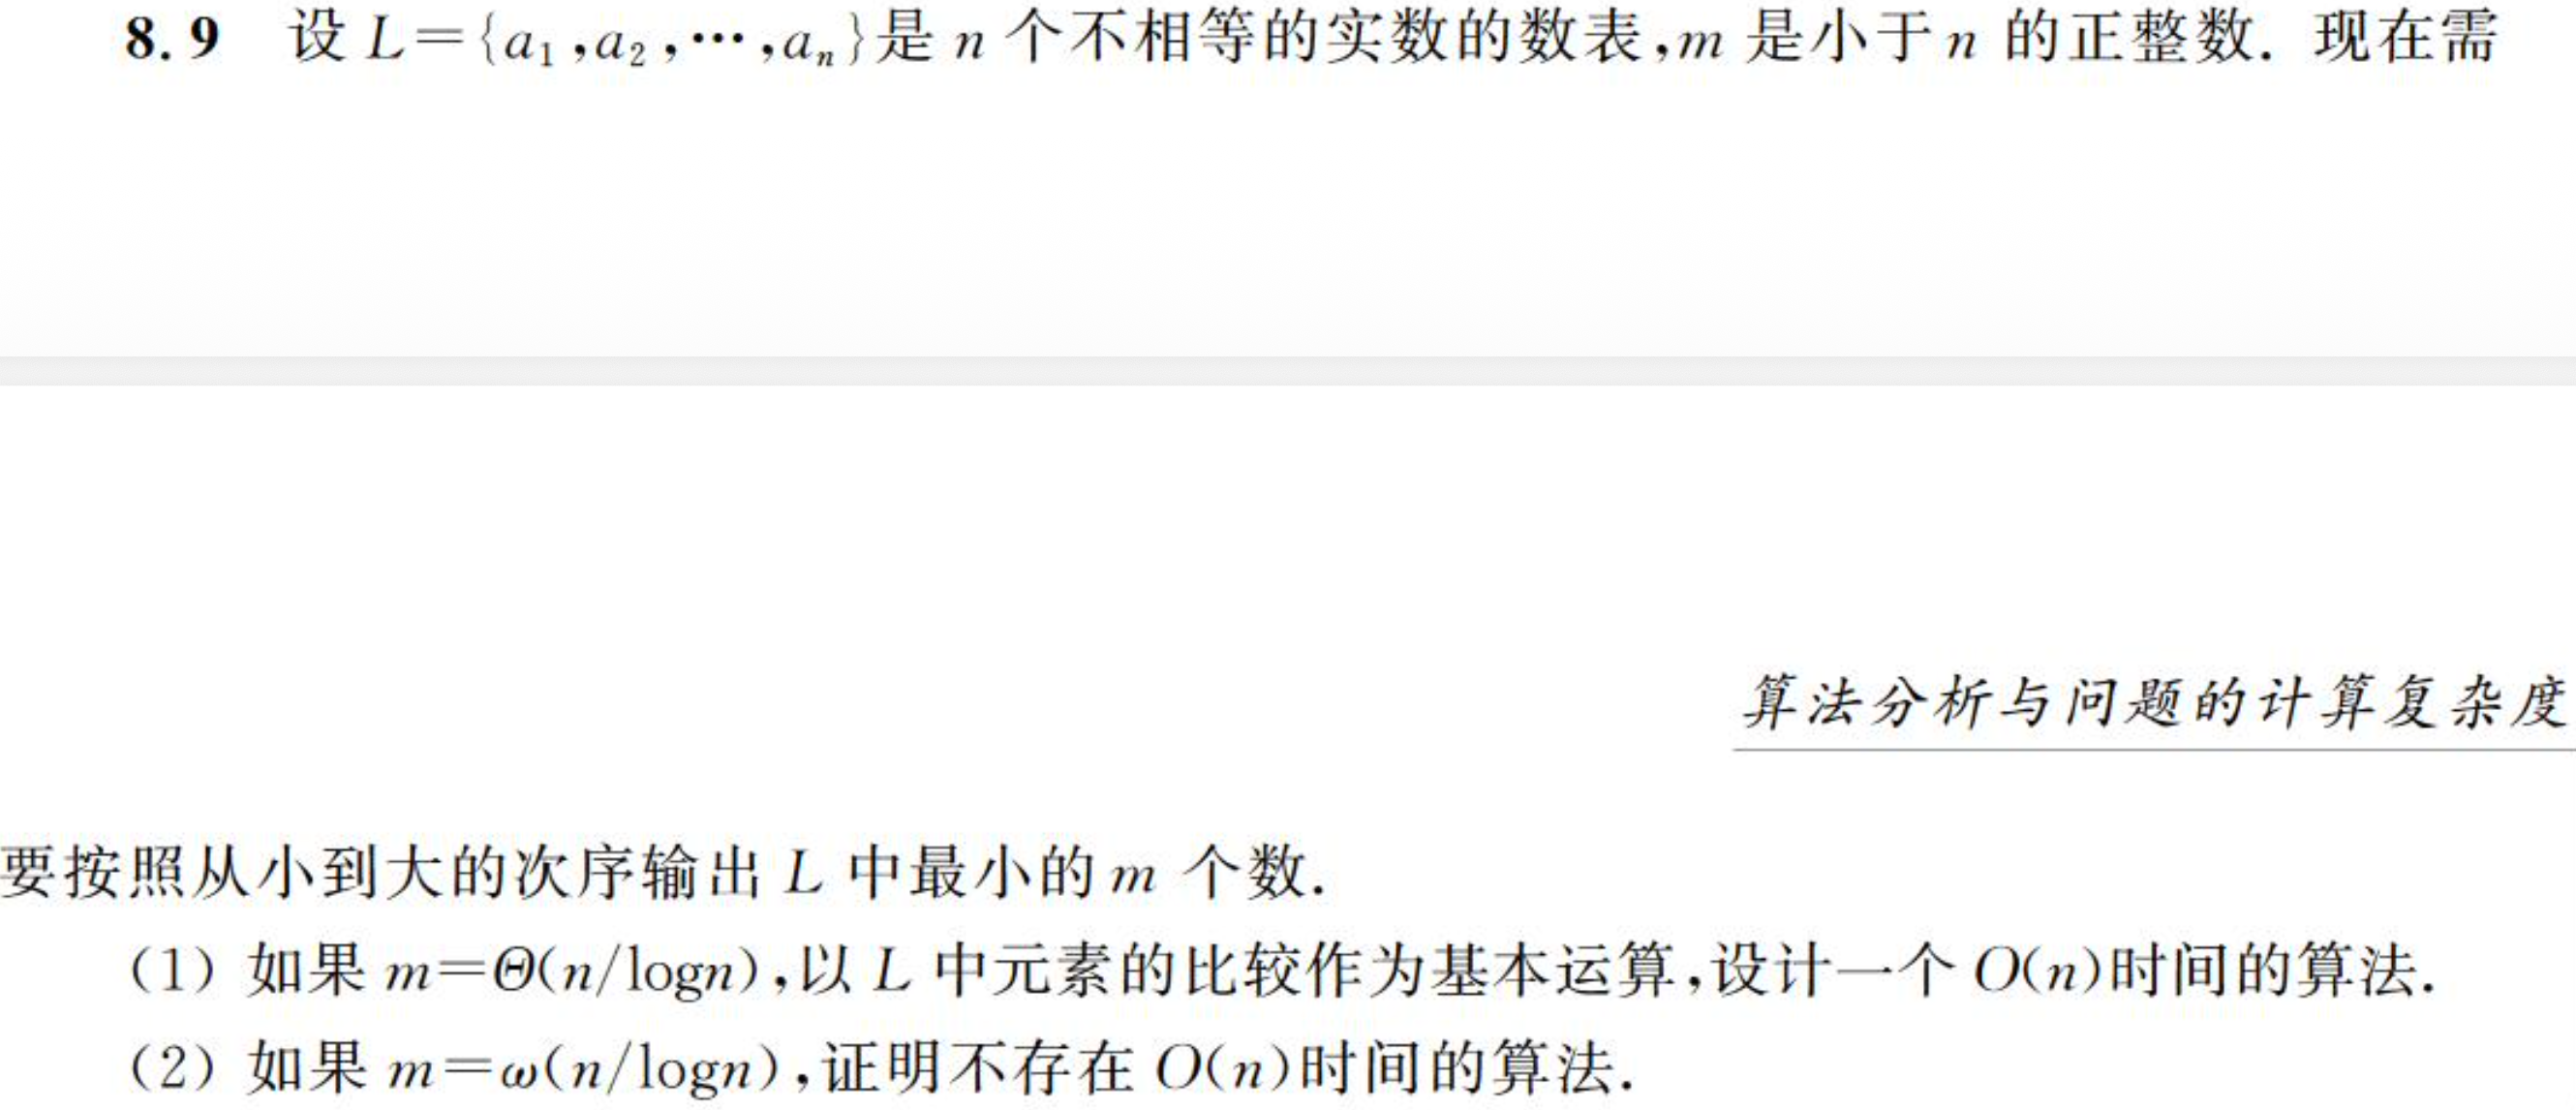
\includegraphics[width=0.6\textwidth]{problems/8.9.png}
\end{center}
\end{problem}

\begin{solution}
(1) 
用线性时间选择算法找到 $L$ 中第 $m$ 小的元素，记为 $x$。

线性时间选择算法可以在最坏情况下用

\[
O(n)
\]

次比较找到第 $m$ 小元素。

扫描整个数表 $L$，找出所有小于等于 $x$ 的元素。

由于 $L$ 中元素互不相等，所以小于等于 $x$ 的元素恰好有 $m$ 个，也就是 $L$ 中最小的 $m$ 个数。

这一步只需一次扫描，时间为

\[
O(n).
\]
对这 $m$ 个元素使用比较排序，例如归并排序或堆排序，然后按从小到大的顺序输出。

排序这 $m$ 个元素需要时间

\[
O(m\log m).
\]

由于

\[
m=\Theta\left(\frac{n}{\log n}\right),
\]

所以

\[
m\log m
=
\Theta\left(\frac{n}{\log n}\log \frac{n}{\log n}\right).
\]

而

\[
\log \frac{n}{\log n}
=
\log n-\log\log n
=
O(\log n),
\]

因此

\[
m\log m
=
O\left(\frac{n}{\log n}\cdot \log n\right)
=
O(n).
\]

所以总时间复杂度为

\[
T(n)
=
O(n)+O(n)+O(m\log m)
=
O(n).
\]

因此，当

\[
m=\Theta\left(\frac{n}{\log n}\right)
\]

时，可以在最坏情况下用

\[
O(n)
\]

时间输出 $L$ 中最小的 $m$ 个数。

(2) 

下面证明：在以比较作为基本运算的模型下，若

\[
m=\omega\left(\frac{n}{\log n}\right),
\]

则不存在最坏情况下时间复杂度为 $O(n)$ 的算法。

因为算法不仅要找出最小的 $m$ 个元素，还要按照从小到大的顺序输出它们。

对于 $n$ 个互不相等的元素，最小的 $m$ 个元素及其相对次序共有

\[
n(n-1)(n-2)\cdots (n-m+1)
=
\frac{n!}{(n-m)!}
\]

种可能。

在比较模型中，任意算法都可以表示为一棵二叉决策树。如果最坏情况下比较次数为 $h$，则决策树高度为 $h$，叶子结点数至多为

\[
2^h.
\]

为了区分所有可能的输出结果，必须有

\[
2^h
\geq
\frac{n!}{(n-m)!}.
\]

因此

\[
h
\geq
\log_2\frac{n!}{(n-m)!}.
\]

下面估计该下界。

若

\[
m\leq \frac n2,
\]

则有

\[
\frac{n!}{(n-m)!}
=
n(n-1)\cdots(n-m+1)
\geq
\left(\frac n2\right)^m.
\]

于是

\[
h
\geq
\log_2\left(\frac n2\right)^m
=
m\log_2\frac n2
=
\Omega(m\log n).
\]

又因为

\[
m=\omega\left(\frac{n}{\log n}\right),
\]

所以

\[
m\log n=\omega(n).
\]

因此

\[
h=\omega(n).
\]

若

\[
m>\frac n2,
\]

则至少需要区分前 $\frac n2$ 小元素的有序输出，因此

\[
h
\geq
\log_2\frac{n!}{(n-\frac n2)!}.
\]

并且

\[
\frac{n!}{(n-\frac n2)!}
=
n(n-1)\cdots\left(\frac n2+1\right)
\geq
\left(\frac n2\right)^{n/2}.
\]

所以

\[
h
\geq
\frac n2\log_2\frac n2
=
\Omega(n\log n).
\]

这当然也有

\[
h=\omega(n).
\]

综上，当

\[
m=\omega\left(\frac{n}{\log n}\right)
\]

时，任何基于比较的算法在最坏情况下都至少需要

\[
\omega(n)
\]

次比较，因此不可能存在最坏情况下时间复杂度为

\[
O(n)
\]

的算法。
\end{solution}

\begin{problem}
\begin{center}
    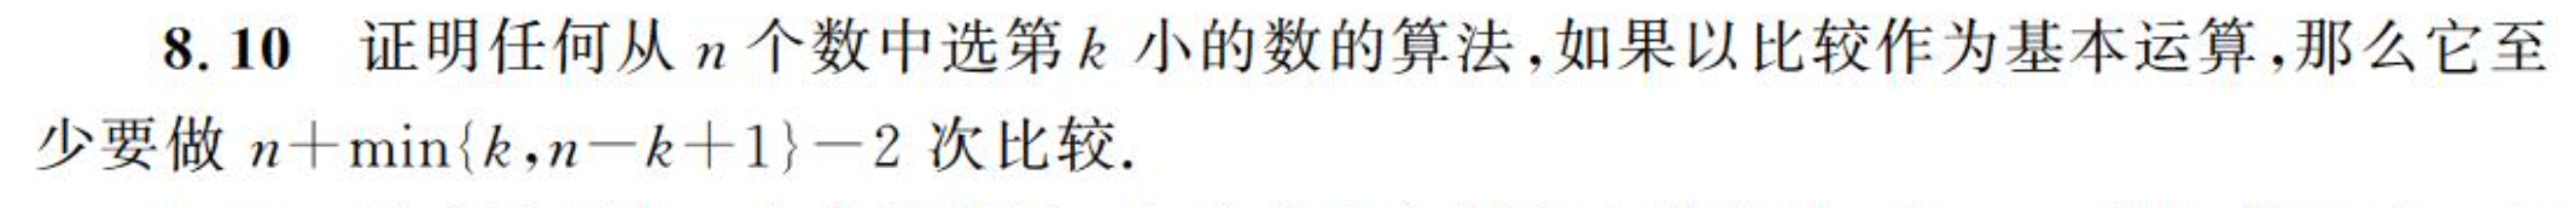
\includegraphics[width=0.6\textwidth]{problems/8.10.png}
\end{center}
\end{problem}

\begin{solution}

证明：任意从 n 个数中选择第 k 小元素的比较算法，

$
最坏情况下至少需要 
n+\min\{k,n-k+1\}-2
次比较。
$

记
\[
r=\min\{k,n-k+1\}.
\]
注意到选择第 \(k\) 小元素与选择第 \(n-k+1\) 大元素是对称的，因此只需证明
\[
k\leq n-k+1
\]
时的下界即可。此时
\[
r=k,
\]
我们要证明任意算法最坏情况下至少需要
\[
n+k-2
\]
次比较。

采用对手论证。

对手将元素分成两类：低类 \(L\) 和高类 \(H\)。对手始终保持如下性质：

\[
\text{低类元素可能排在第 } k \text{ 小元素之前，}
\]
\[
\text{高类元素可能排在第 } k \text{ 小元素之后。}
\]

在比较过程中，对手尽量使算法无法同时获得两方面的信息。具体地说：

\[
\text{每次比较至多只能排除一个元素成为第 } k \text{ 小元素的可能性。}
\]

首先，要确定第 \(k\) 小元素，算法必须证明有 \(n-k\) 个元素比它大。否则，如果少于 \(n-k\) 个元素被证明比某个候选元素大，那么该候选元素仍然可能排在第 \(k\) 小之后，算法无法确定答案。

因此，至少需要

\[
n-k
\]

次比较来排除这 \(n-k\) 个较大的元素。

另一方面，算法还必须证明有 \(k-1\) 个元素比第 \(k\) 小元素小。否则，如果不能确定有 \(k-1\) 个元素在它之前，那么该元素也可能不是第 \(k\) 小。

这又至少需要

\[
k-1
\]

次比较。

仅有上述两部分信息还不够。因为第 \(k\) 小元素本身必须同时与“小于它的一侧”和“大于它的一侧”建立比较关系。换言之，在比较决策树中，最终被输出的元素必须既能与前面的 \(k-1\) 个元素区分开，又能与后面的 \(n-k\) 个元素区分开。

在对手策略下，这额外需要至少

\[
k-1
\]

次比较。直观地说，当 \(k\leq n-k+1\) 时，较小的一侧规模为 \(k\)，算法至少要在这 \(k\) 个可能较小的元素中确定最大的那个；而确定 \(k\) 个元素中的最大者至少需要

\[
k-1
\]

次比较。

于是总比较次数至少为

\[
(n-k)+(k-1)+(k-1).
\]

化简得

\[
(n-k)+(k-1)+(k-1)
=
n+k-2.
\]

因此，当

\[
k\leq n-k+1
\]

时，任意比较算法在最坏情况下至少需要

\[
n+k-2
\]

次比较。

同理，当

\[
k>n-k+1
\]

时，可以对称地考虑选择第 \(n-k+1\) 大元素。此时较小的一侧规模变为

\[
n-k+1,
\]

于是最坏情况下至少需要

\[
n+(n-k+1)-2
\]

次比较。

综上，任意从 \(n\) 个数中选择第 \(k\) 小元素的比较算法，最坏情况下至少需要

\[
\boxed{
n+\min\{k,n-k+1\}-2
}
\]

次比较。
\end{solution}


\end{document}